\documentclass[12pt]{article}

\usepackage[margin=1in]{geometry}
\usepackage{amsmath}
\usepackage{amsfonts}
\usepackage{amssymb}
\usepackage{graphicx}
\usepackage{booktabs}
\usepackage{float}
\usepackage{hyperref}
\usepackage{cite}
\usepackage{rotating}
\usepackage{subcaption}

\newcommand{\E}{\mathbb{E}}
\newcommand{\Var}{\mathbb{V}}

\title{MGTECON 603 - Problem Set 5\\ \small{(Instructor: Guido Imbens)}}
\author{Wooyong Park\\ {\small Collaborators: Cem Kozanoglu, Roberto Gonzalez Tellez, Hanniel Ho, Aileen Wu}}
\date{\today}


\begin{document}

\maketitle

\section*{0 Summary Statistics}

The summary statistics of the data are shown in table \ref{tab:summary_stats} in the appendix.
Also, the scatterplot and the correlation matrix of the data are shown in figures \ref{fig:scatterplot_matrix} and \ref{fig:correlation_matrix_plot} in the appendix.

\section{Problem 1}

\subsection{Regression of re78 on re75}

The regression result of re78 on re75 is shown in table \ref{tab:regression_re75}, which is visualized in figure \ref{fig:scatterplot_re75_re78}.

The high R-squared values suggest that re75 is a good predictor of re78 with the regression coefficient being $0.6955$(p-value: $<$ 0.001).

\begin{figure}[h]
    \centering
    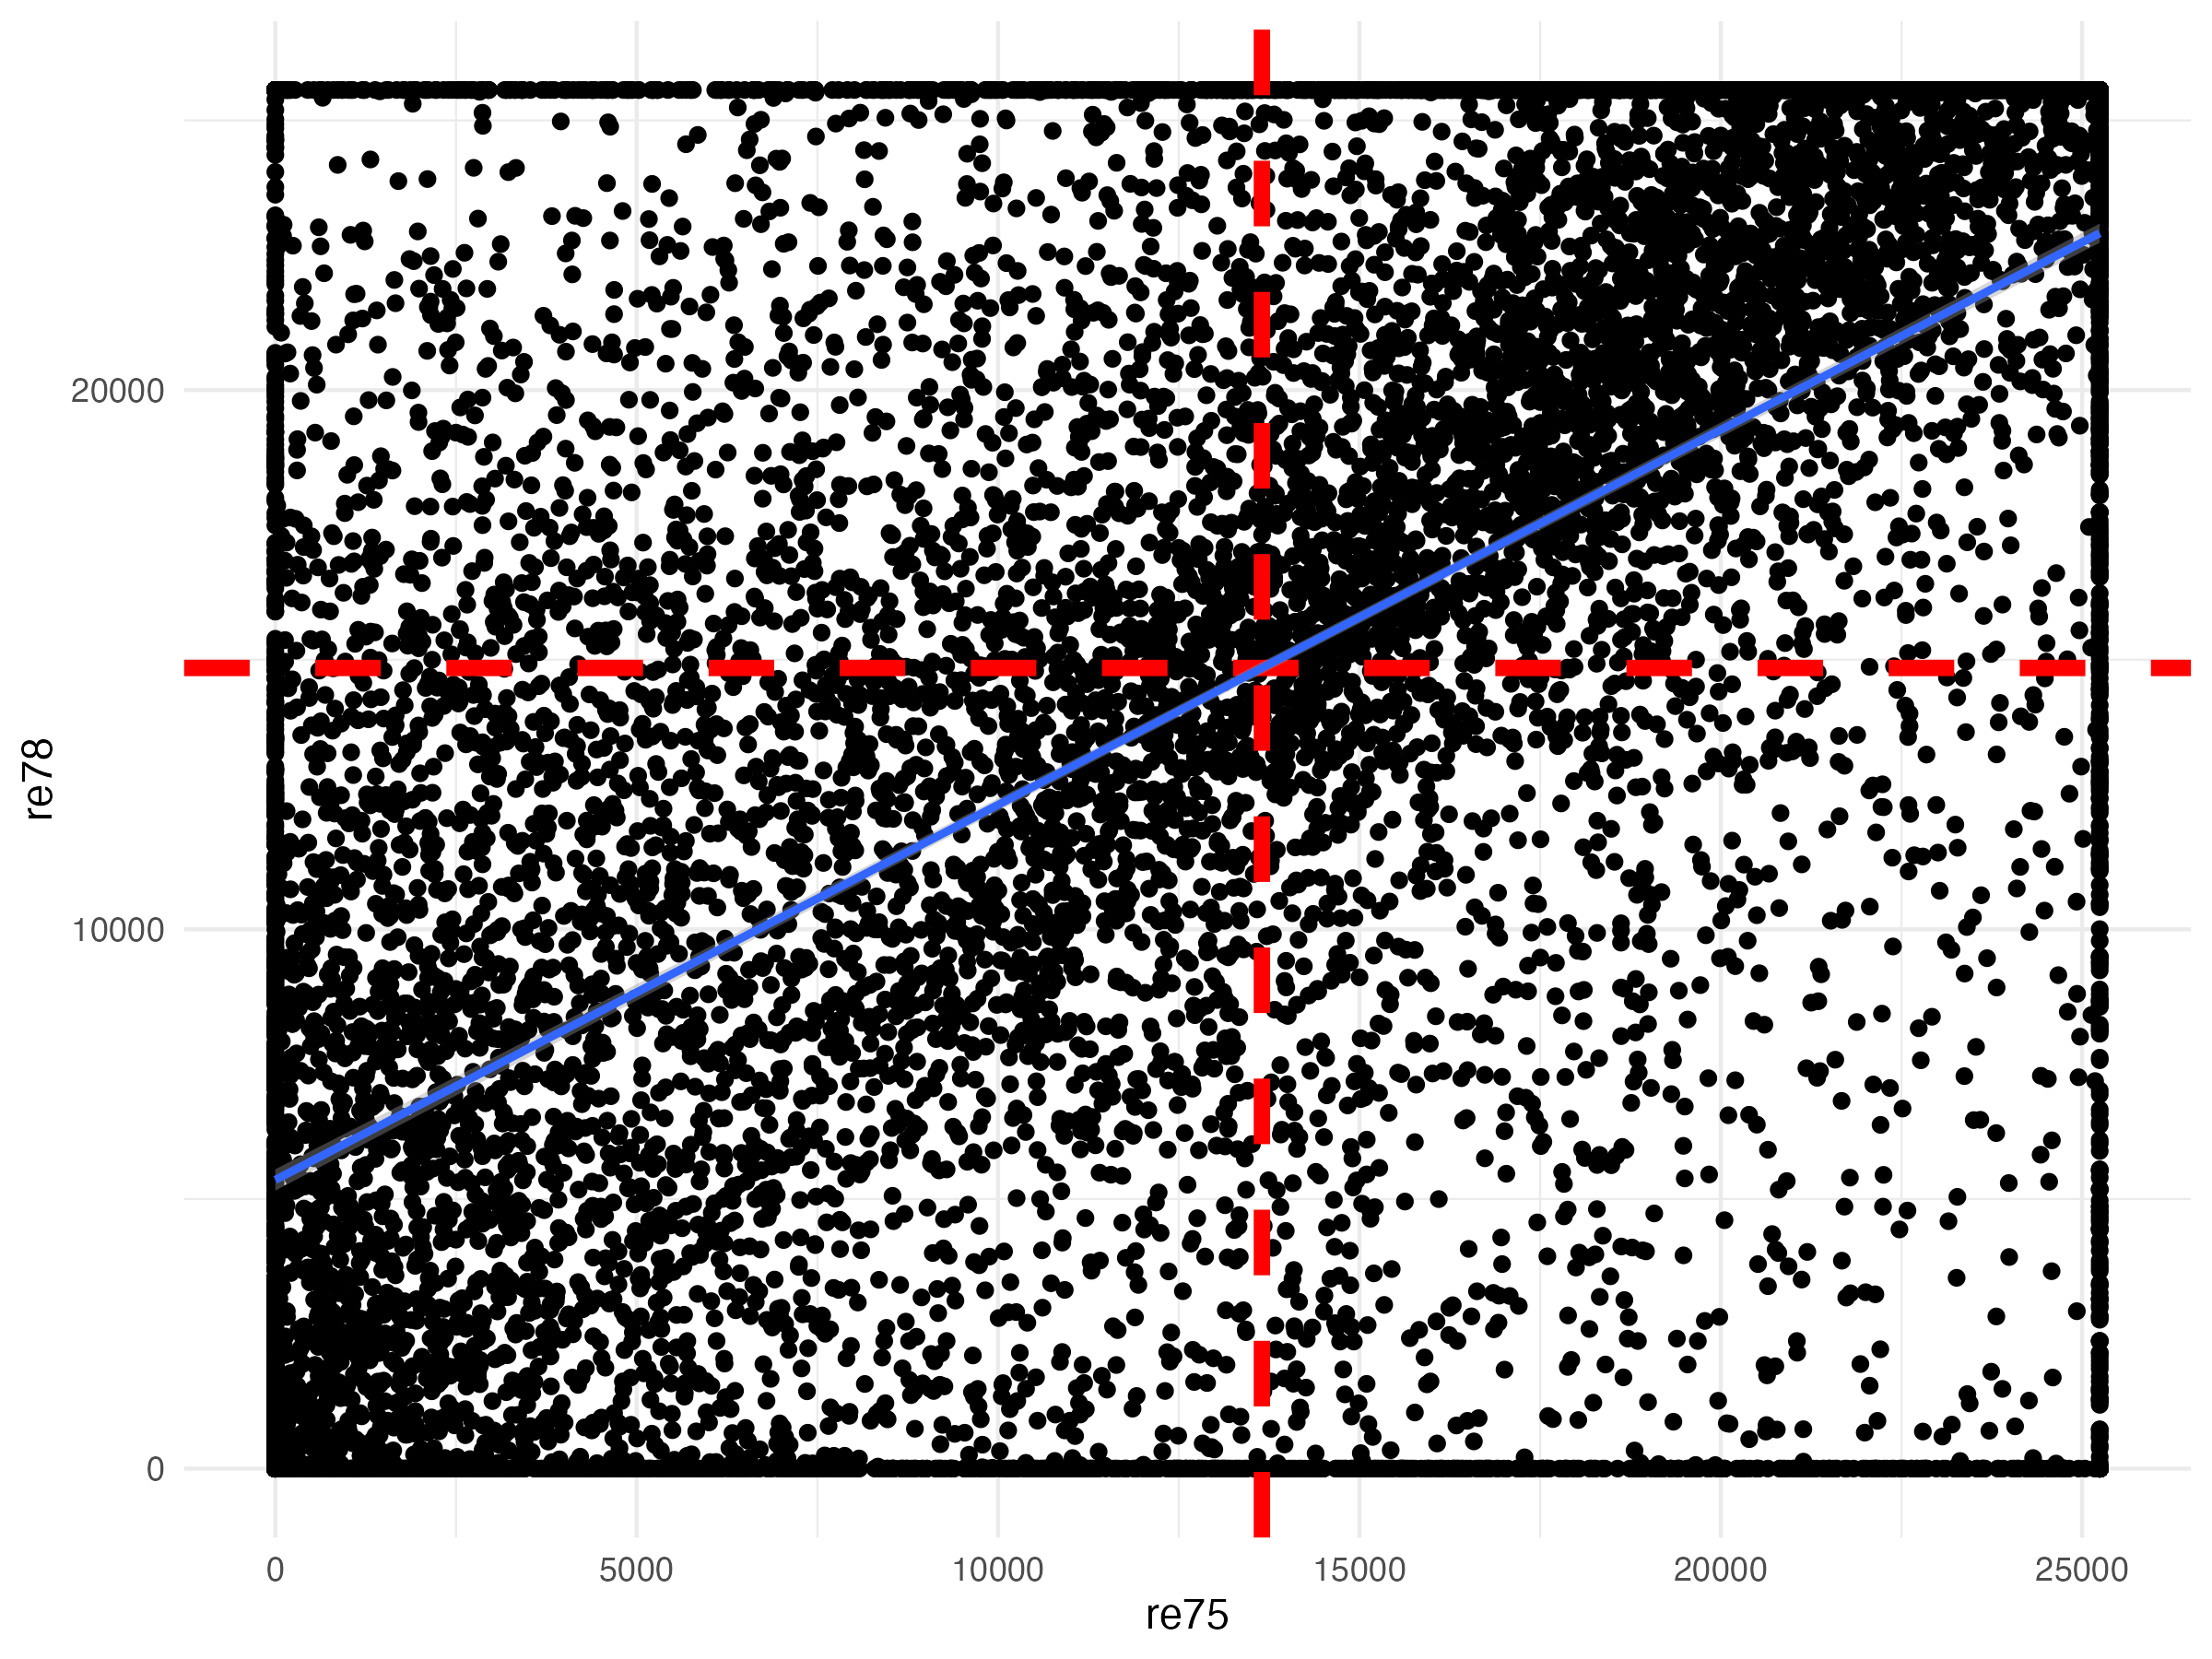
\includegraphics[width=0.8\textwidth]{output/scatterplot_re75_re78.png}
    \caption{\label{fig:scatterplot_re75_re78}Scatterplot of re75 and re78}
    \begin{minipage}{\textwidth}
        \footnotesize
        Notes: The plot shows the scatterplot of re75 and re78. The line is the regression line. Also note that these earnings have a clear maximum and minimum cutoffs, which make the plot display a strict rectangle form.
        This is potentially due to winsorization done on the data.
        The red dashed lines indicate the mean of re75 and re78.
        \end{minipage}
\end{figure}


\begin{table}[h]
\begin{center}
\begin{tabular}{l c}
\hline
 & Model 1 \\
\hline
(Intercept)             & $5352.7055^{***}$ \\
                        & $(100.8683)$      \\
re75                    & $0.6955^{***}$    \\
                        & $(0.0060)$        \\
\hline
Num. obs.               & $15992$           \\
R$^2$ (full model)      & $0.4466$          \\
R$^2$ (proj model)      & $$                \\
Adj. R$^2$ (full model) & $0.4466$          \\
Adj. R$^2$ (proj model) & $$                \\
\hline
\multicolumn{2}{l}{\scriptsize{$^{***}p<0.01$; $^{**}p<0.05$; $^{*}p<0.1$}}
\end{tabular}
\caption{Regression of re78 on re75}
\label{tab:regression_re75}
\end{center}
\end{table}


\subsection{Leverage of re75}

The leverage equation for single covariate case is given by:
\begin{align}
    h_i &= \frac{1}{n} + \frac{(x_i - \overline{x})^2}{\sum_{j=1}^n (x_j - \overline{x})^2}
\end{align}

where $i$ is the index of observation, $x_i$ is the value of the covariate, and $\overline{x}$ is the mean of the covariate.
This suggests that the end points of the data are the observations with the highest leverage.
Since the mean is closer to the right end point of re75, it is likely that the observations at the left end(i.e., the ones with the lowest re75) are the ones with the highest leverage.
The table \ref{tab:highest_leverage_re75} shows the top 5 observations with the highest leverage, which are consistent with the above observation – the observations with the lowest re75(i.e., zero) have the highest leverage.

% latex table generated in R 4.4.3 by xtable 1.8-4 package
% Tue Nov 11 06:59:54 2025
\begin{table}[ht]
\centering
\begin{tabular}{rrr}
  \hline
 & re75 & leverage\_re75 \\ 
  \hline
1 & 0.000000 & 0.000198 \\ 
  2 & 0.000000 & 0.000198 \\ 
  3 & 0.000000 & 0.000198 \\ 
  4 & 0.000000 & 0.000198 \\ 
  5 & 0.000000 & 0.000198 \\ 
   \hline
\end{tabular}
\caption{Top 5 observations with the highest leverage(single regressor)} 
\label{tab:highest_leverage_re75}
\end{table}


This can be also seen in figure \ref{fig:scatterplot_re75_leverage_re75}, which shows the scatterplot of re75 and its leverage. The plot is U-shaped with the lowest re75 having the highest leverage, which is consistent with the above observation.
\begin{figure}[h]
    \centering
    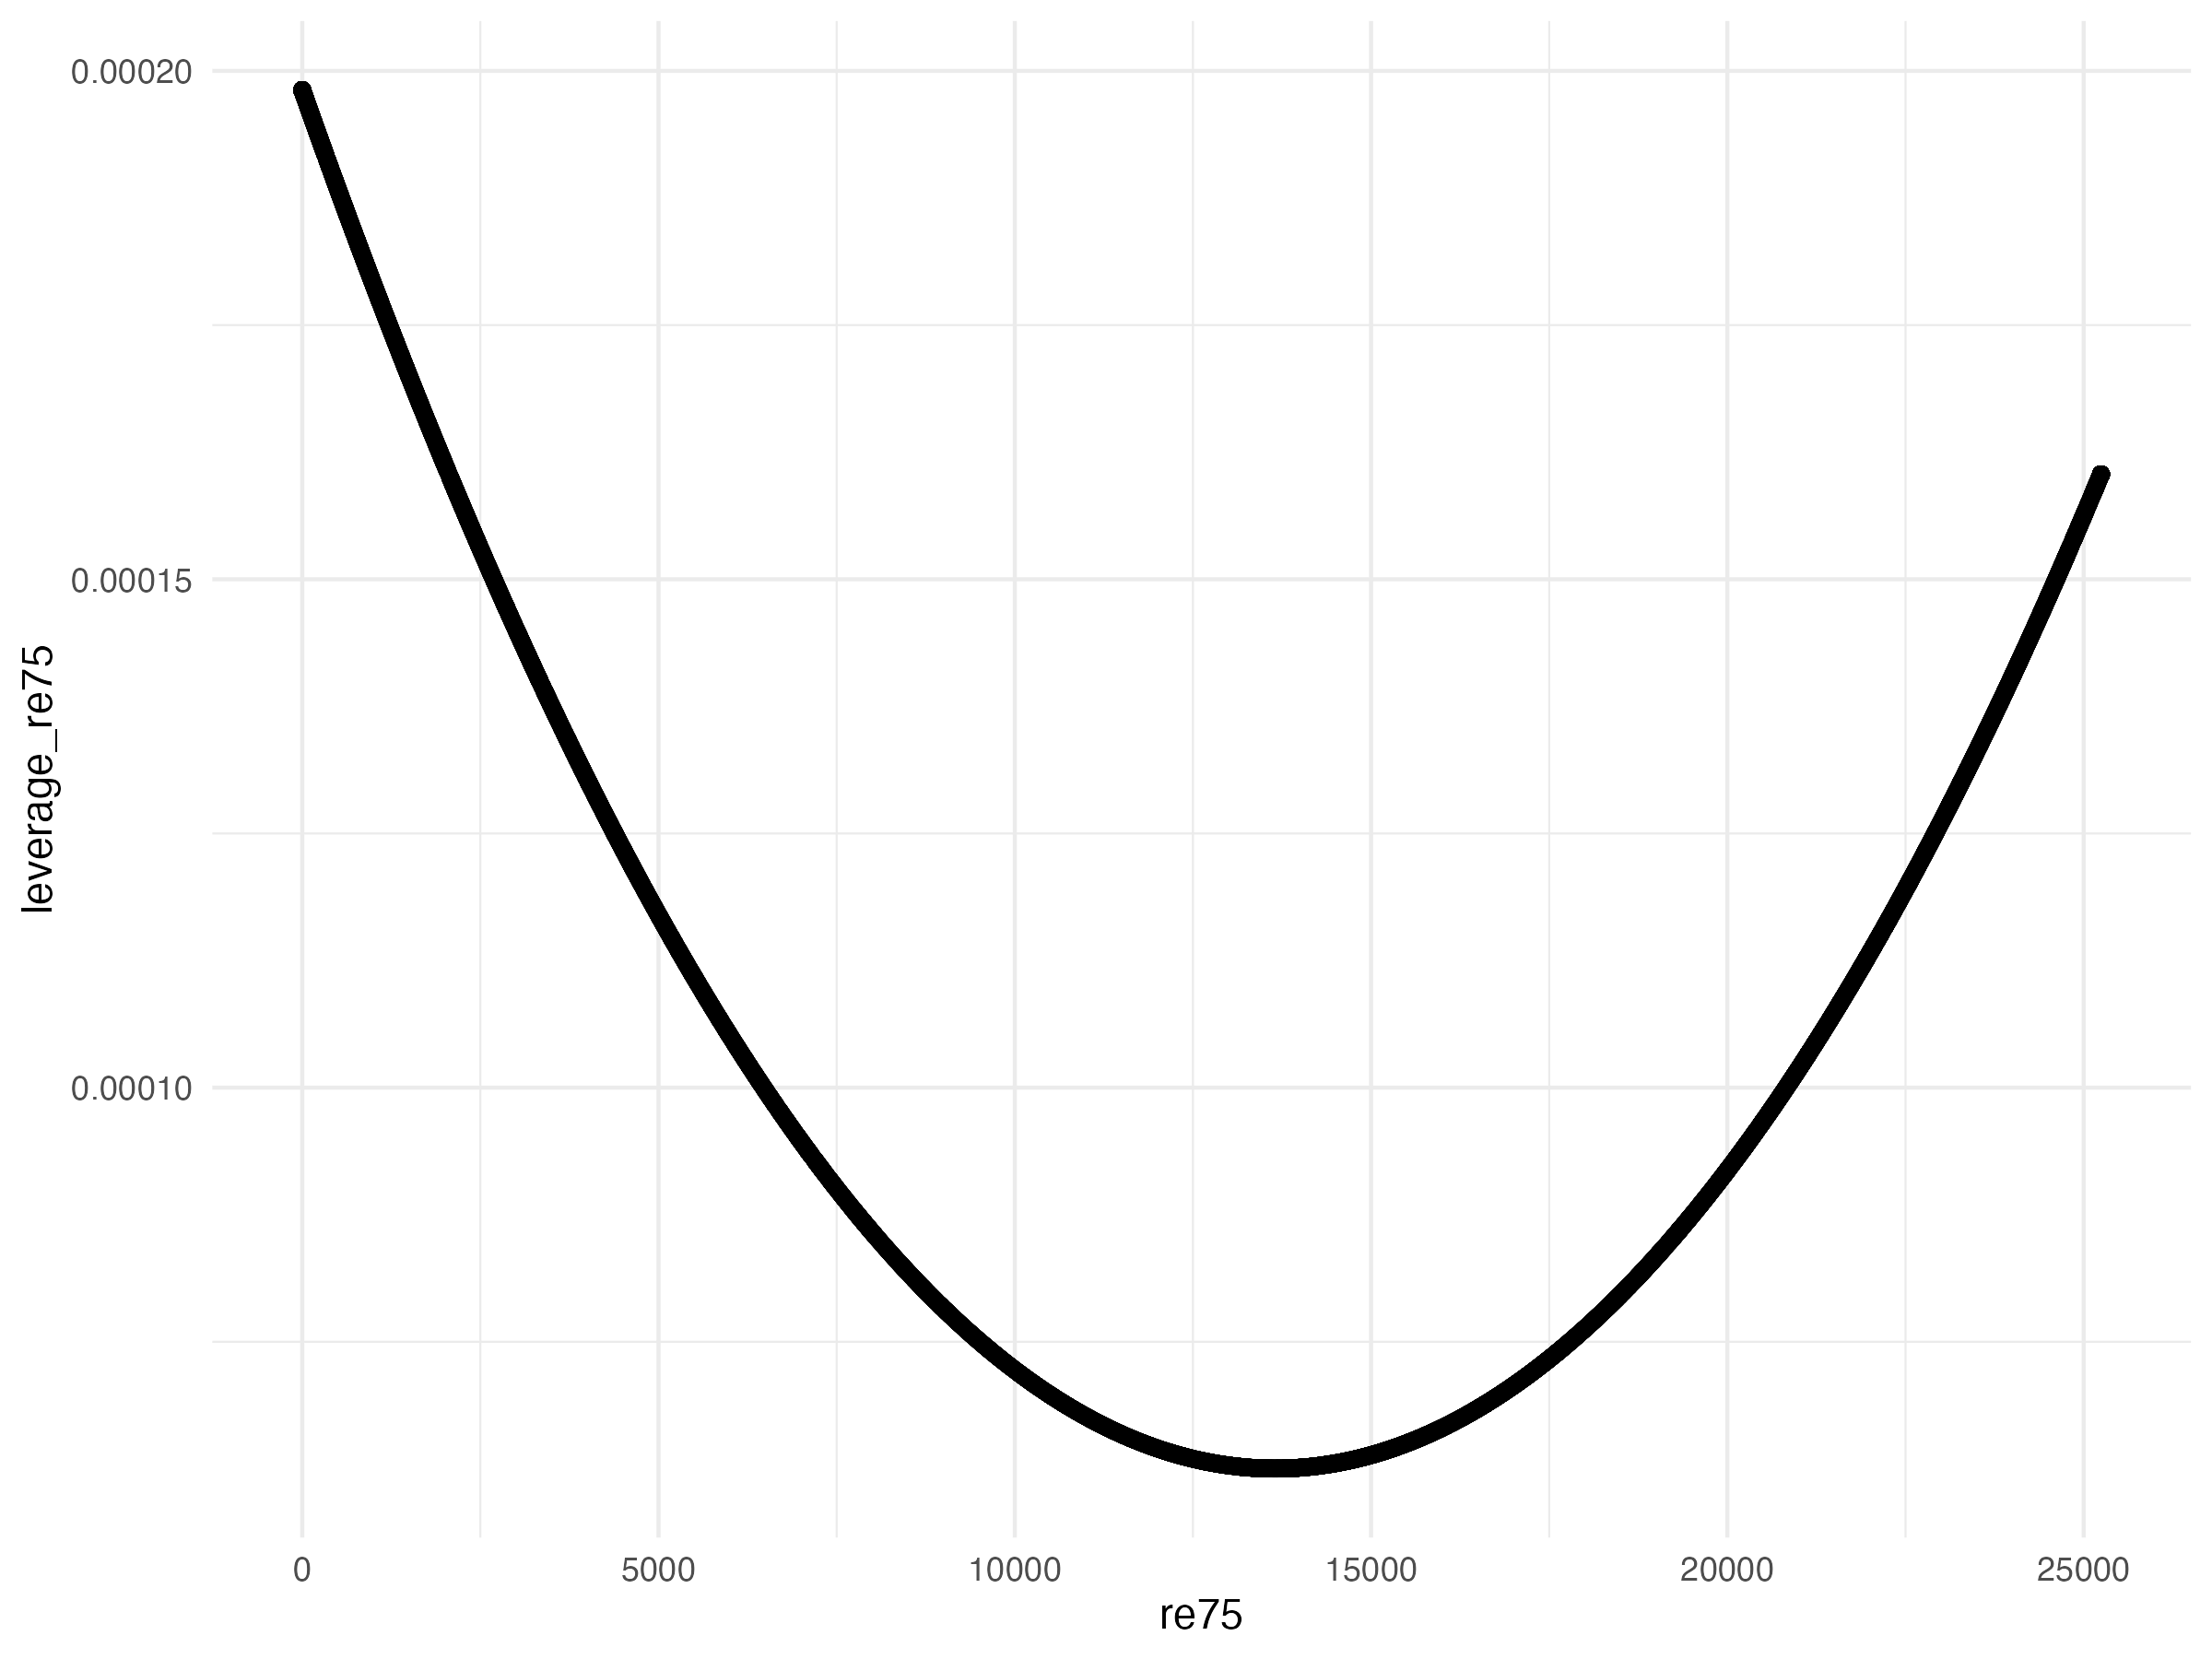
\includegraphics[width=0.6\textwidth]{output/scatterplot_re75_leverage_re75.png}
    \caption{\label{fig:scatterplot_re75_leverage_re75}Scatterplot of re75 and its leverage}
\end{figure}

\section{Problem 2}
\subsection{Regression of re78 on re75, re74, education, black, hispanic, and age}

The regression result of re78 on re75, re74, education, black, hispanic, and age is shown in table \ref{tab:regression_re75_re74_education_black_hispanic_age}.


\begin{table}[h]
\begin{center}
\begin{tabular}{l c}
\hline
 & Model 1 \\
\hline
(Intercept)             & $6461.5815^{***}$ \\
                        & $(306.6338)$      \\
re75                    & $0.4702^{***}$    \\
                        & $(0.0153)$        \\
re74                    & $0.2913^{***}$    \\
                        & $(0.0150)$        \\
education               & $113.9149^{***}$  \\
                        & $(20.2172)$       \\
black                   & $-826.2451^{***}$ \\
                        & $(198.3461)$      \\
hispanic                & $-209.0108$       \\
                        & $(218.7439)$      \\
age                     & $-102.6443^{***}$ \\
                        & $(5.3389)$        \\
\hline
Num. obs.               & $15992$           \\
R$^2$ (full model)      & $0.4752$          \\
R$^2$ (proj model)      & $$                \\
Adj. R$^2$ (full model) & $0.4750$          \\
Adj. R$^2$ (proj model) & $$                \\
\hline
\multicolumn{2}{l}{\scriptsize{$^{***}p<0.01$; $^{**}p<0.05$; $^{*}p<0.1$}}
\end{tabular}
\caption{Regression of re78 on re75, re74, education, black, hispanic, and age}
\label{tab:regression_re75_re74_education_black_hispanic_age}
\end{center}
\end{table}


The regression results indicate that past earnings (re75 and re74) and education level are significant positive predictors of earnings in 1978. Conversely, being Black and older age are associated with significantly lower earnings, while being Hispanic does not have a statistically significant effect.

\subsection{Leverage of re75, re74, education, black, hispanic, and age}

The leverage equation for multiple covariates case is given by:
\begin{align}
    [\mathbf{H}]_{ii} &= \biggl[\mathbf{X}\bigl(\mathbf{X}'\mathbf{X}\bigr)^{-1}\mathbf{X}'\biggr]_{ii}
\end{align}

where $i$ is the index of observation, $x_i$ is the value of the covariate, and $\overline{x}$ is the mean of the covariate.
This suggests that the end points of the data are the observations with the highest leverage.
Since the mean is closer to the right end point of re75, it is likely that the observations at the left end(i.e., the ones with the lowest re75) are the ones with the highest leverage.
The table \ref{tab:highest_leverage_re75_re74_education_black_hispanic_age} shows the top 5 observations with the highest leverage, which are consistent with the above observation – the observations with the lowest re75(i.e., zero) have the highest leverage.

The five observations with the highest leverage are shown in table \ref{tab:highest_leverage_re75_re74_education_black_hispanic_age}. 
The last column(high\_leverage) indicates whether the observation is a high leverage observation, defined as leverage value greater than $3K/n$, where $K$ is the number of covariates and $n$ is the number of observations.
Although the cutoff is quite arbitrary, the five observations with the highest leverage are all high leverage observations.

\textbf{Is this concerning?} I do think so according to the cutoff. \textbf{What concerns me more} is that the data seems to have been winsorized, which is potentially due to the outliers.
However, given that the winsorized numbers would all fall into the group of high leverage observations, I believe that this implies that the winsorization cutoff is what drives the regression results.

% latex table generated in R 4.4.3 by xtable 1.8-4 package
% Tue Nov 11 06:59:55 2025
\begin{table}[ht]
\centering
\begin{tabular}{rrrrl}
  \hline
 & re75 & re74 & leverage\_multivariate & high\_leverage \\ 
  \hline
1 & 25243.5500 & 0.0000 & 0.0030 & TRUE \\ 
  2 & 25243.5500 & 0.0000 & 0.0027 & TRUE \\ 
  3 & 1090.3060 & 25862.3200 & 0.0026 & TRUE \\ 
  4 & 25243.5500 & 0.0000 & 0.0026 & TRUE \\ 
  5 & 25241.7600 & 0.0000 & 0.0026 & TRUE \\ 
   \hline
\end{tabular}
\caption{Top 5 observations with the highest leverage(multiple regressors)} 
\label{tab:highest_leverage_re75_re74_education_black_hispanic_age}
\end{table}



\section{Problem 3}

\subsection{Residuals and their Standardization}

Figure \ref{fig:histogram_standardized_residuals_problem_3} shows the histogram of the standardized residuals.
\begin{figure}[h]
    \centering
    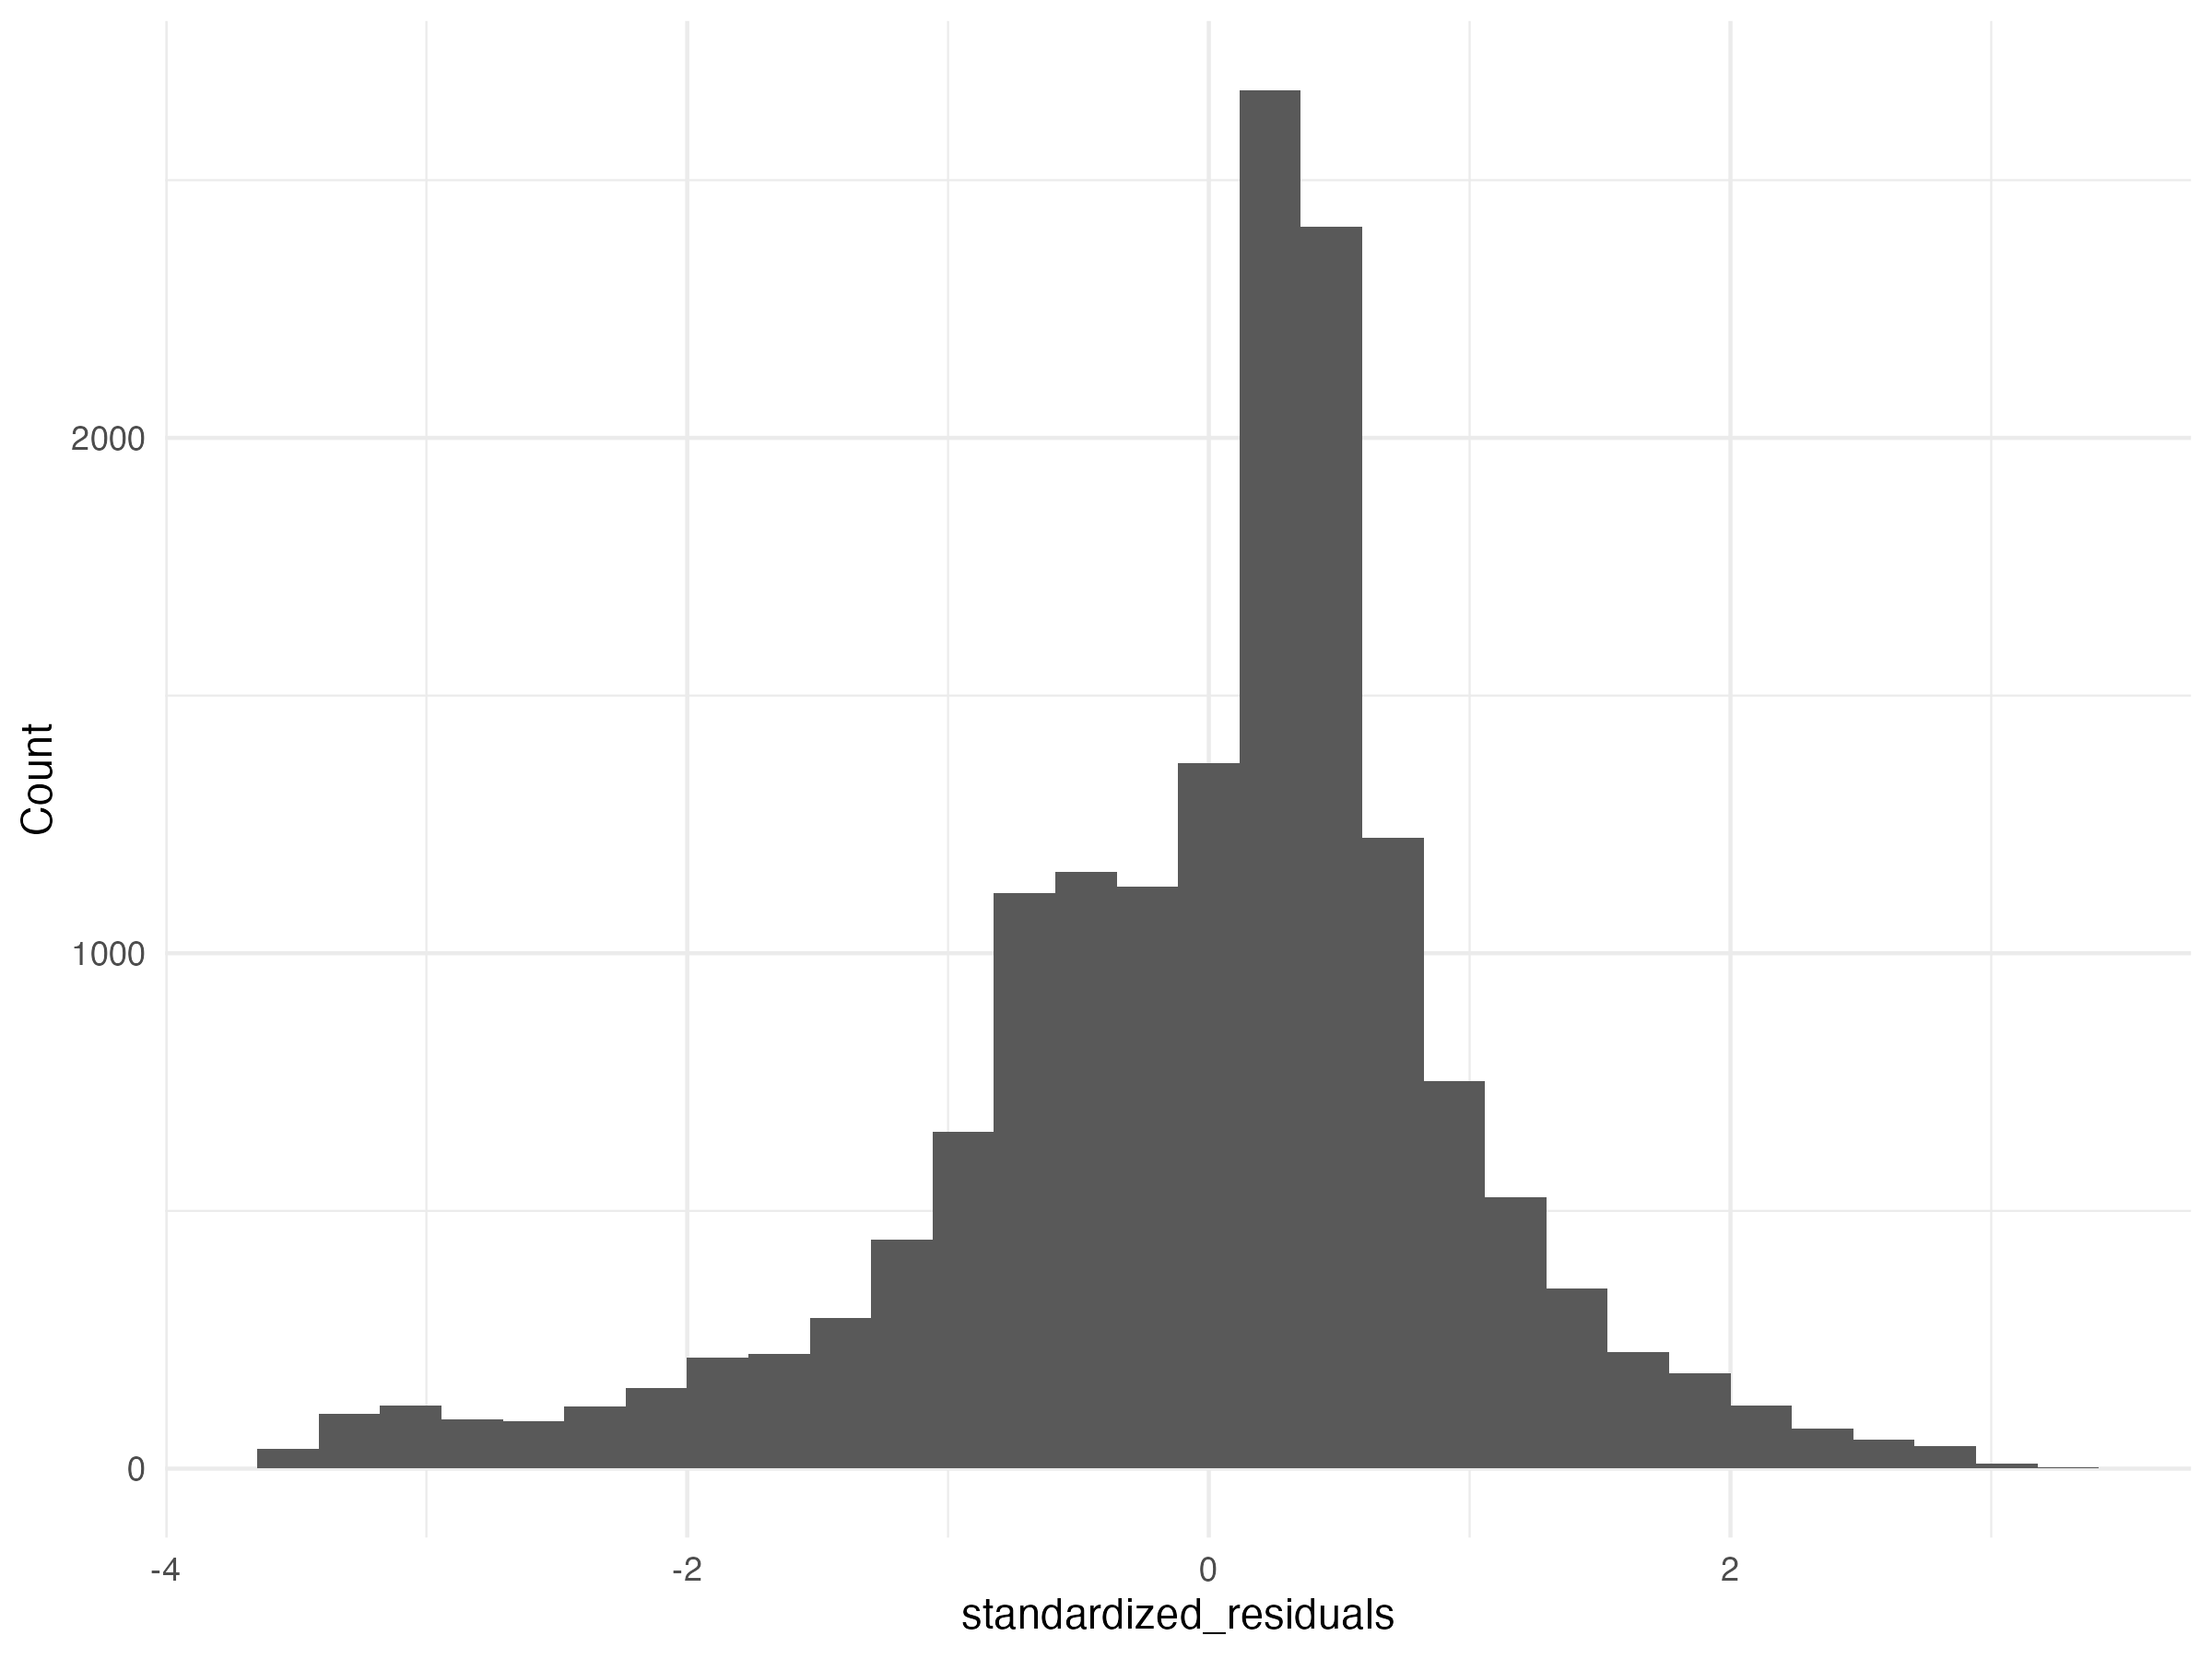
\includegraphics[width=0.7\textwidth]{output/histogram_standardized_residuals_problem_3.png}
    \caption{\label{fig:histogram_standardized_residuals_problem_3}Histogram of the standardized residuals}
\end{figure}

The highest five values in absolute value are shown in table \ref{tab:highest_standardized_residuals}. Here, we do not have any observations from the top 5 observations with the highest leverage.
This is likely due to the fact that high leverage observations generally have lower conditional variance of the residuals\footnote{conditional on the covariates}, and thus the residuals with higher absolute value are less likely to be high leverage observations.

% latex table generated in R 4.4.3 by xtable 1.8-4 package
% Tue Nov 11 06:59:55 2025
\begin{table}[ht]
\centering
\begin{tabular}{rrrrl}
  \hline
 & id & abs\_standardized\_residuals & leverage\_multivariate & high\_leverage \\ 
  \hline
1 &  9670 & 3.5681 & 0.0004 & FALSE \\ 
  2 & 12499 & 3.5438 & 0.0003 & FALSE \\ 
  3 &  3810 & 3.5364 & 0.0003 & FALSE \\ 
  4 & 13754 & 3.5355 & 0.0003 & FALSE \\ 
  5 & 12173 & 3.5307 & 0.0003 & FALSE \\ 
   \hline
\end{tabular}
\caption{Top 5 observations with the highest absolute standardized residuals} 
\label{tab:highest_standardized_residuals}
\end{table}


\section{Problem 4}
\subsection{10-fold Cross-Validation}

For problems 4 and 5, I use 10 fold cross-validation to estimate the RMSE of the model.
In detail, the overall out-of-sample RMSE is estimated as follows:
\begin{enumerate}
    \item \textbf{Partition the Data}: The entire dataset is randomly shuffled and divided into 10 equally sized, non-overlapping subsets, often called ``folds". Let these folds be denoted as $F_1, F_2, \ldots, F_{10}$.
    Given a specific fold $F_k$, denote the remaining 9 folds as $F_{-k}$.
    \item \textbf{Iterative Training and Testing}: A loop is executed 10 times. In each iteration $k$ (from 1 to 10):
    \begin{itemize}
        \item Fit the model on the training set $F_{-k}$: $$\arg\min_{\beta^{(-k)}} \sum_{i \in F_{-k}} (y_i - \beta^{(-k)\top} x_i)^2$$
        \item The trained model is then used to predict the outcomes for the observations in the held-out fold, $F_k$: $$\hat{y}_i = \beta^{(-k)\top} x_i$$
    \end{itemize}
    \item \textbf{Compute Overall RMSE}: Finally, the out-of-sample RMSE is calculated by aggregating the prediction errors from all 10 folds.
\end{enumerate}

The formula is:
\begin{align}
    RMSE_{CV} &= \sqrt{\frac{1}{n} \sum_{i=1}^n (y_i - \hat{y}_i)^2}
\end{align}

where $y_i$ is the true outcome for observation $i$, and $\hat{y}_i$ is the out-of-sample prediction for observation $i$ that was generated when its fold was used as the test set.


\subsection{Simple Regression and OOS RMSE}

The RMSE that I obtained from the simple regression is 7177.183. This result is derived by the following code:

\begin{verbatim}
k_folds <- 10
data$fold <- sample(1:k_folds, n, replace = TRUE)
all_predictions_p4 <- data.table()
    
for (k in 1:k_folds) {
    train_data <- data[fold != k]
    test_data <- data[fold == k]
      
    ## Fit the model
    l <- fixest::feols(fml = as.formula(paste0("re78 ~ re75")), 
                        data = train_data, 
                        vcov = "hetero")
      
    predictions <- test_data[, predicted_re78 := predict(l, newdata = test_data)]
      
    temp_data <- data.table(id = test_data$id, 
                            re78 = test_data$re78, 
                            predicted_re78 = predictions)
    all_predictions_p4 <- rbind(all_predictions_p4, temp_data)
    }
    
all_predictions_p4[, error := re78 - predicted_re78]
RMSE_p4 <- sqrt(mean(all_predictions_p4$error^2))
\end{verbatim}

The scatter plot of predictions and errors is shown in figure \ref{fig:scatterplot_predicted_re78_error_p4_cv}.

\begin{figure}[h]
    \centering
    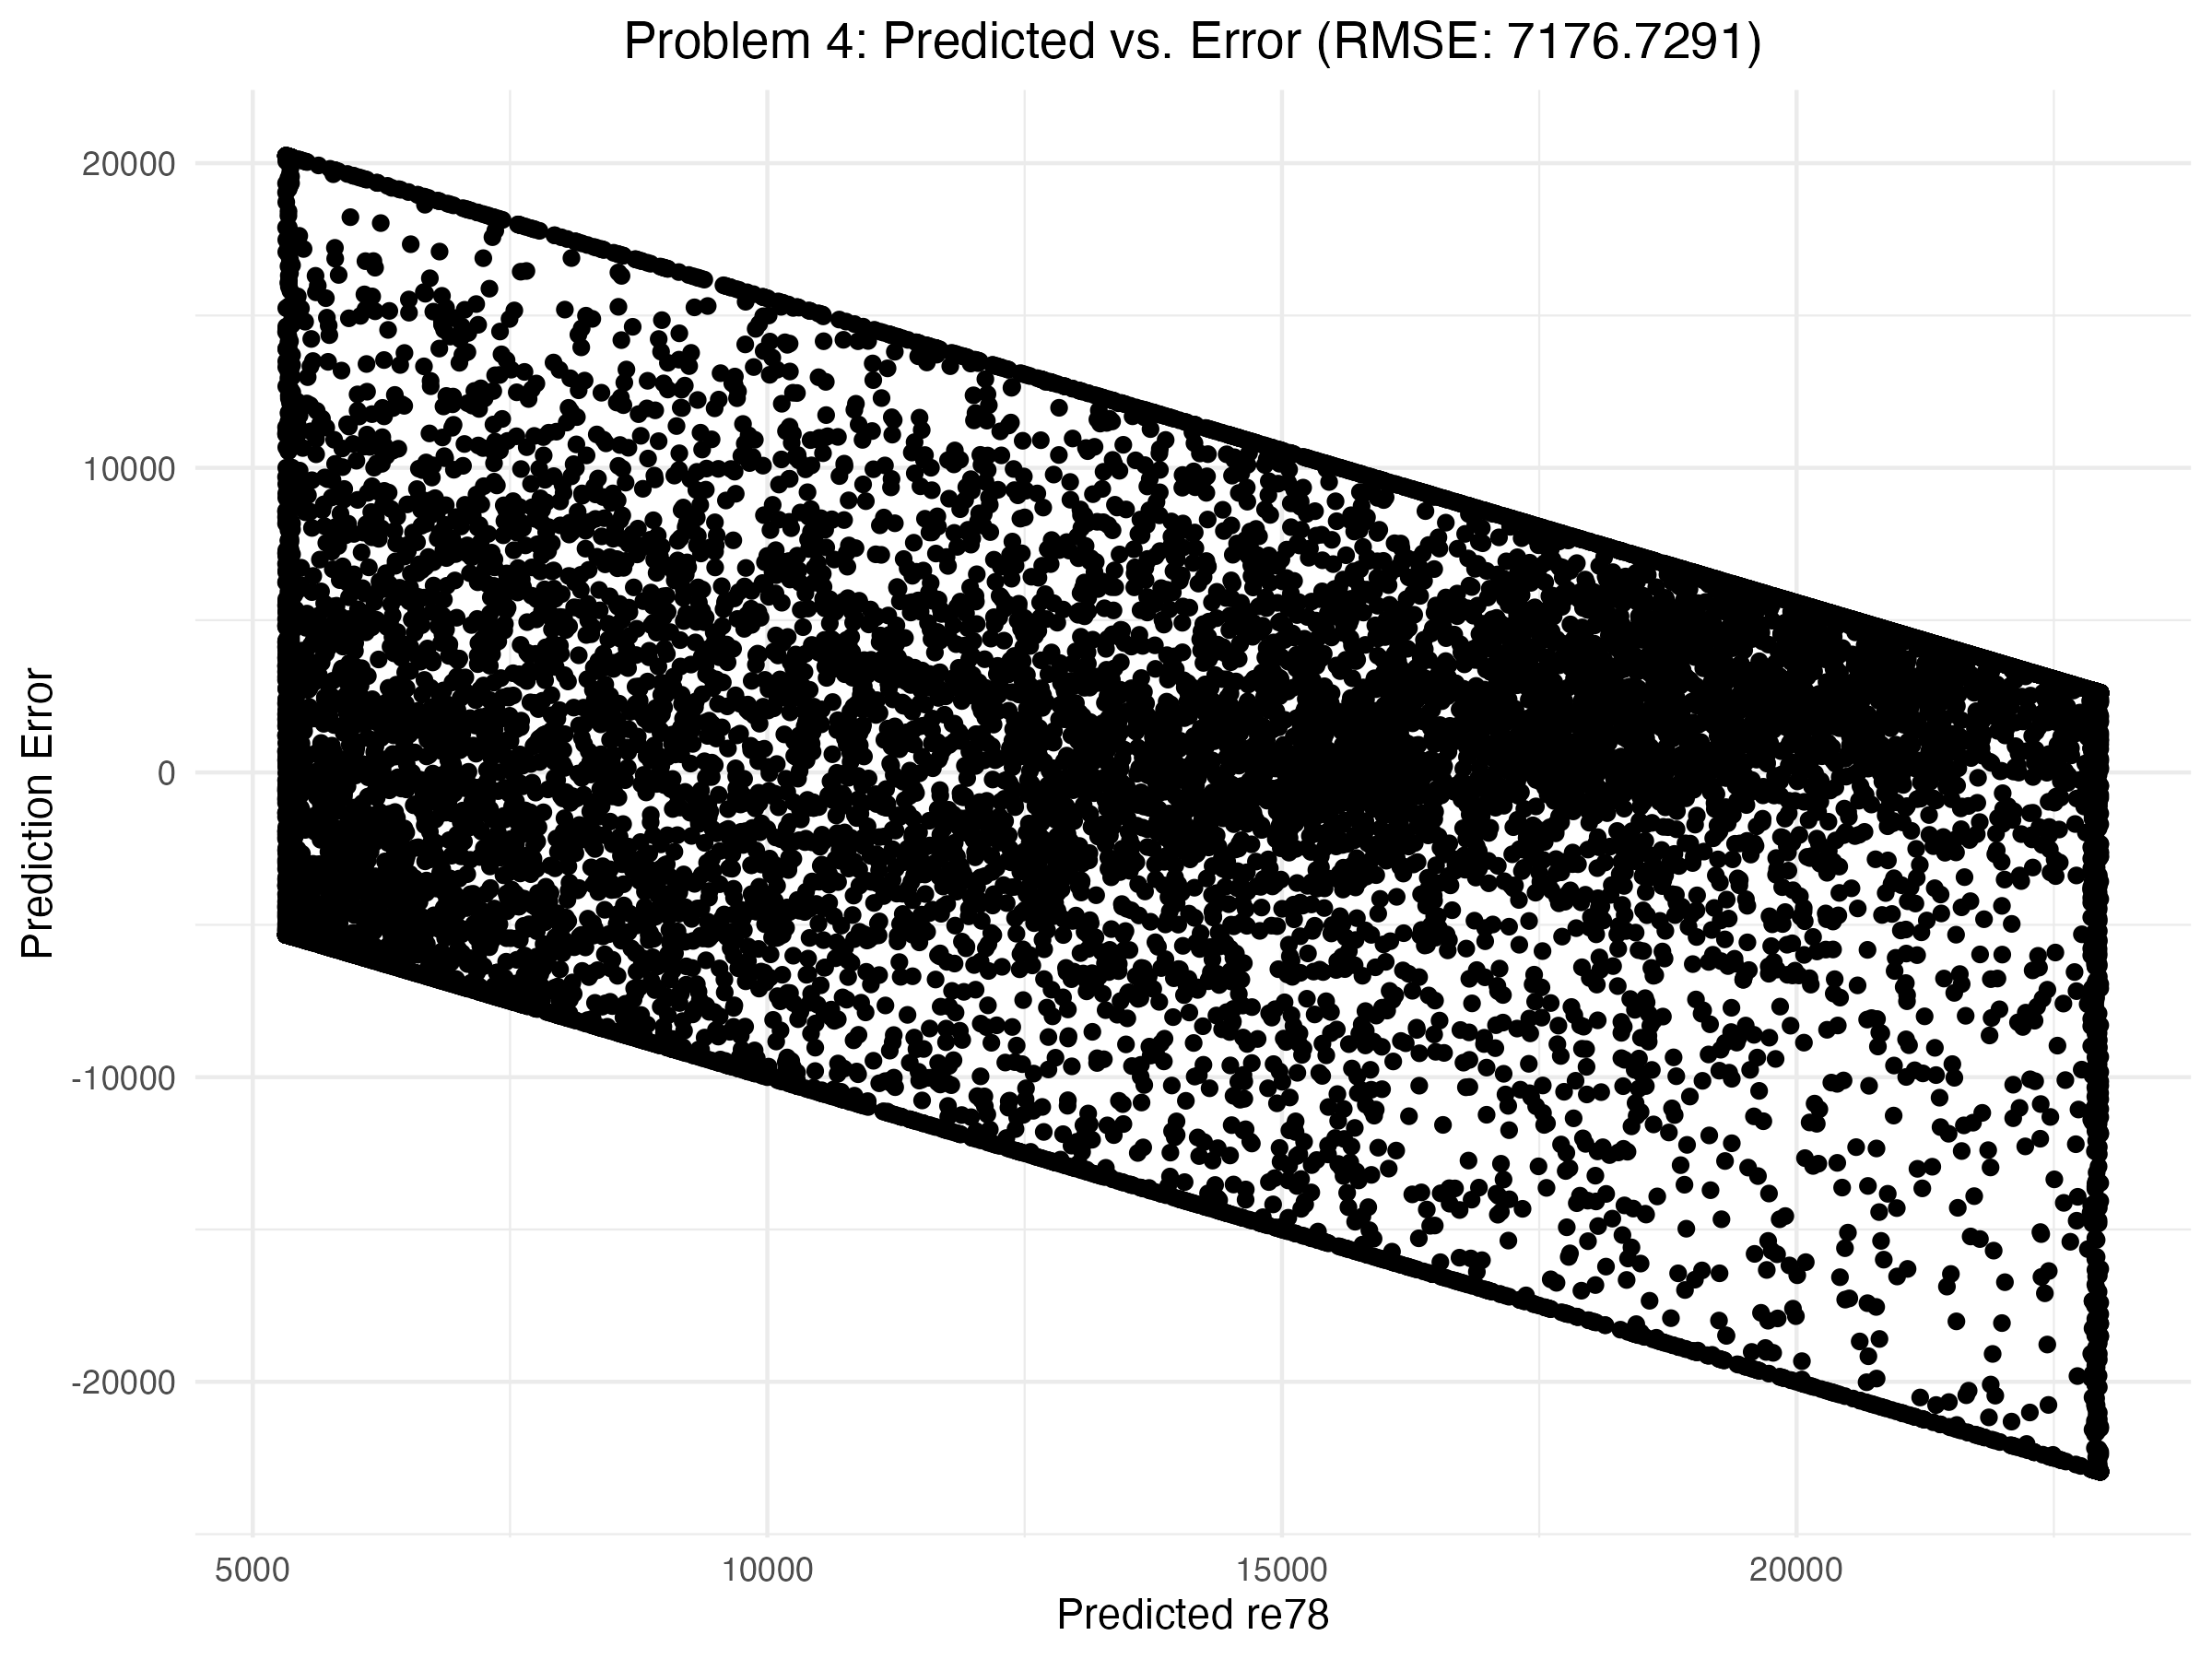
\includegraphics[width=0.8\textwidth]{output/scatterplot_predicted_re78_error_p4_cv.png}
    \caption{\label{fig:scatterplot_predicted_re78_error_p4_cv}Scatterplot of predicted re78 and error}
\end{figure}


\section{Problem 5}

\subsection{Multiple Regression and OOS RMSE}
The RMSE that I obtained from the multiple regression is 6691.683. This result is derived by the following code:

\begin{verbatim}
all_predictions_p5 <- data.table()

for (k in 1:k_folds) {
    train_data <- data[fold != k]
    test_data <- data[fold == k]
      
    rhs <- "re75 + re74 + education + black + hispanic + age"
      
    ## Fit the model
    l <- fixest::feols(fml = as.formula(paste0("re78 ~ ", rhs)), 
                        data = train_data, 
                        vcov = "hetero")
      
    predictions <- predict(l, newdata = test_data)
      
    temp_data <- data.table(id = test_data$id, 
                            re78 = test_data$re78, 
                            predicted_re78 = predictions)
    all_predictions_p5 <- rbind(all_predictions_p5, temp_data)
    }
    
    all_predictions_p5[, error := re78 - predicted_re78]
    RMSE_p5 <- sqrt(mean(all_predictions_p5$error^2))
\end{verbatim}

The scatter plot of predictions and errors is shown in figure \ref{fig:scatterplot_predicted_re78_error_p5_cv}.

\begin{figure}[h]
    \centering
    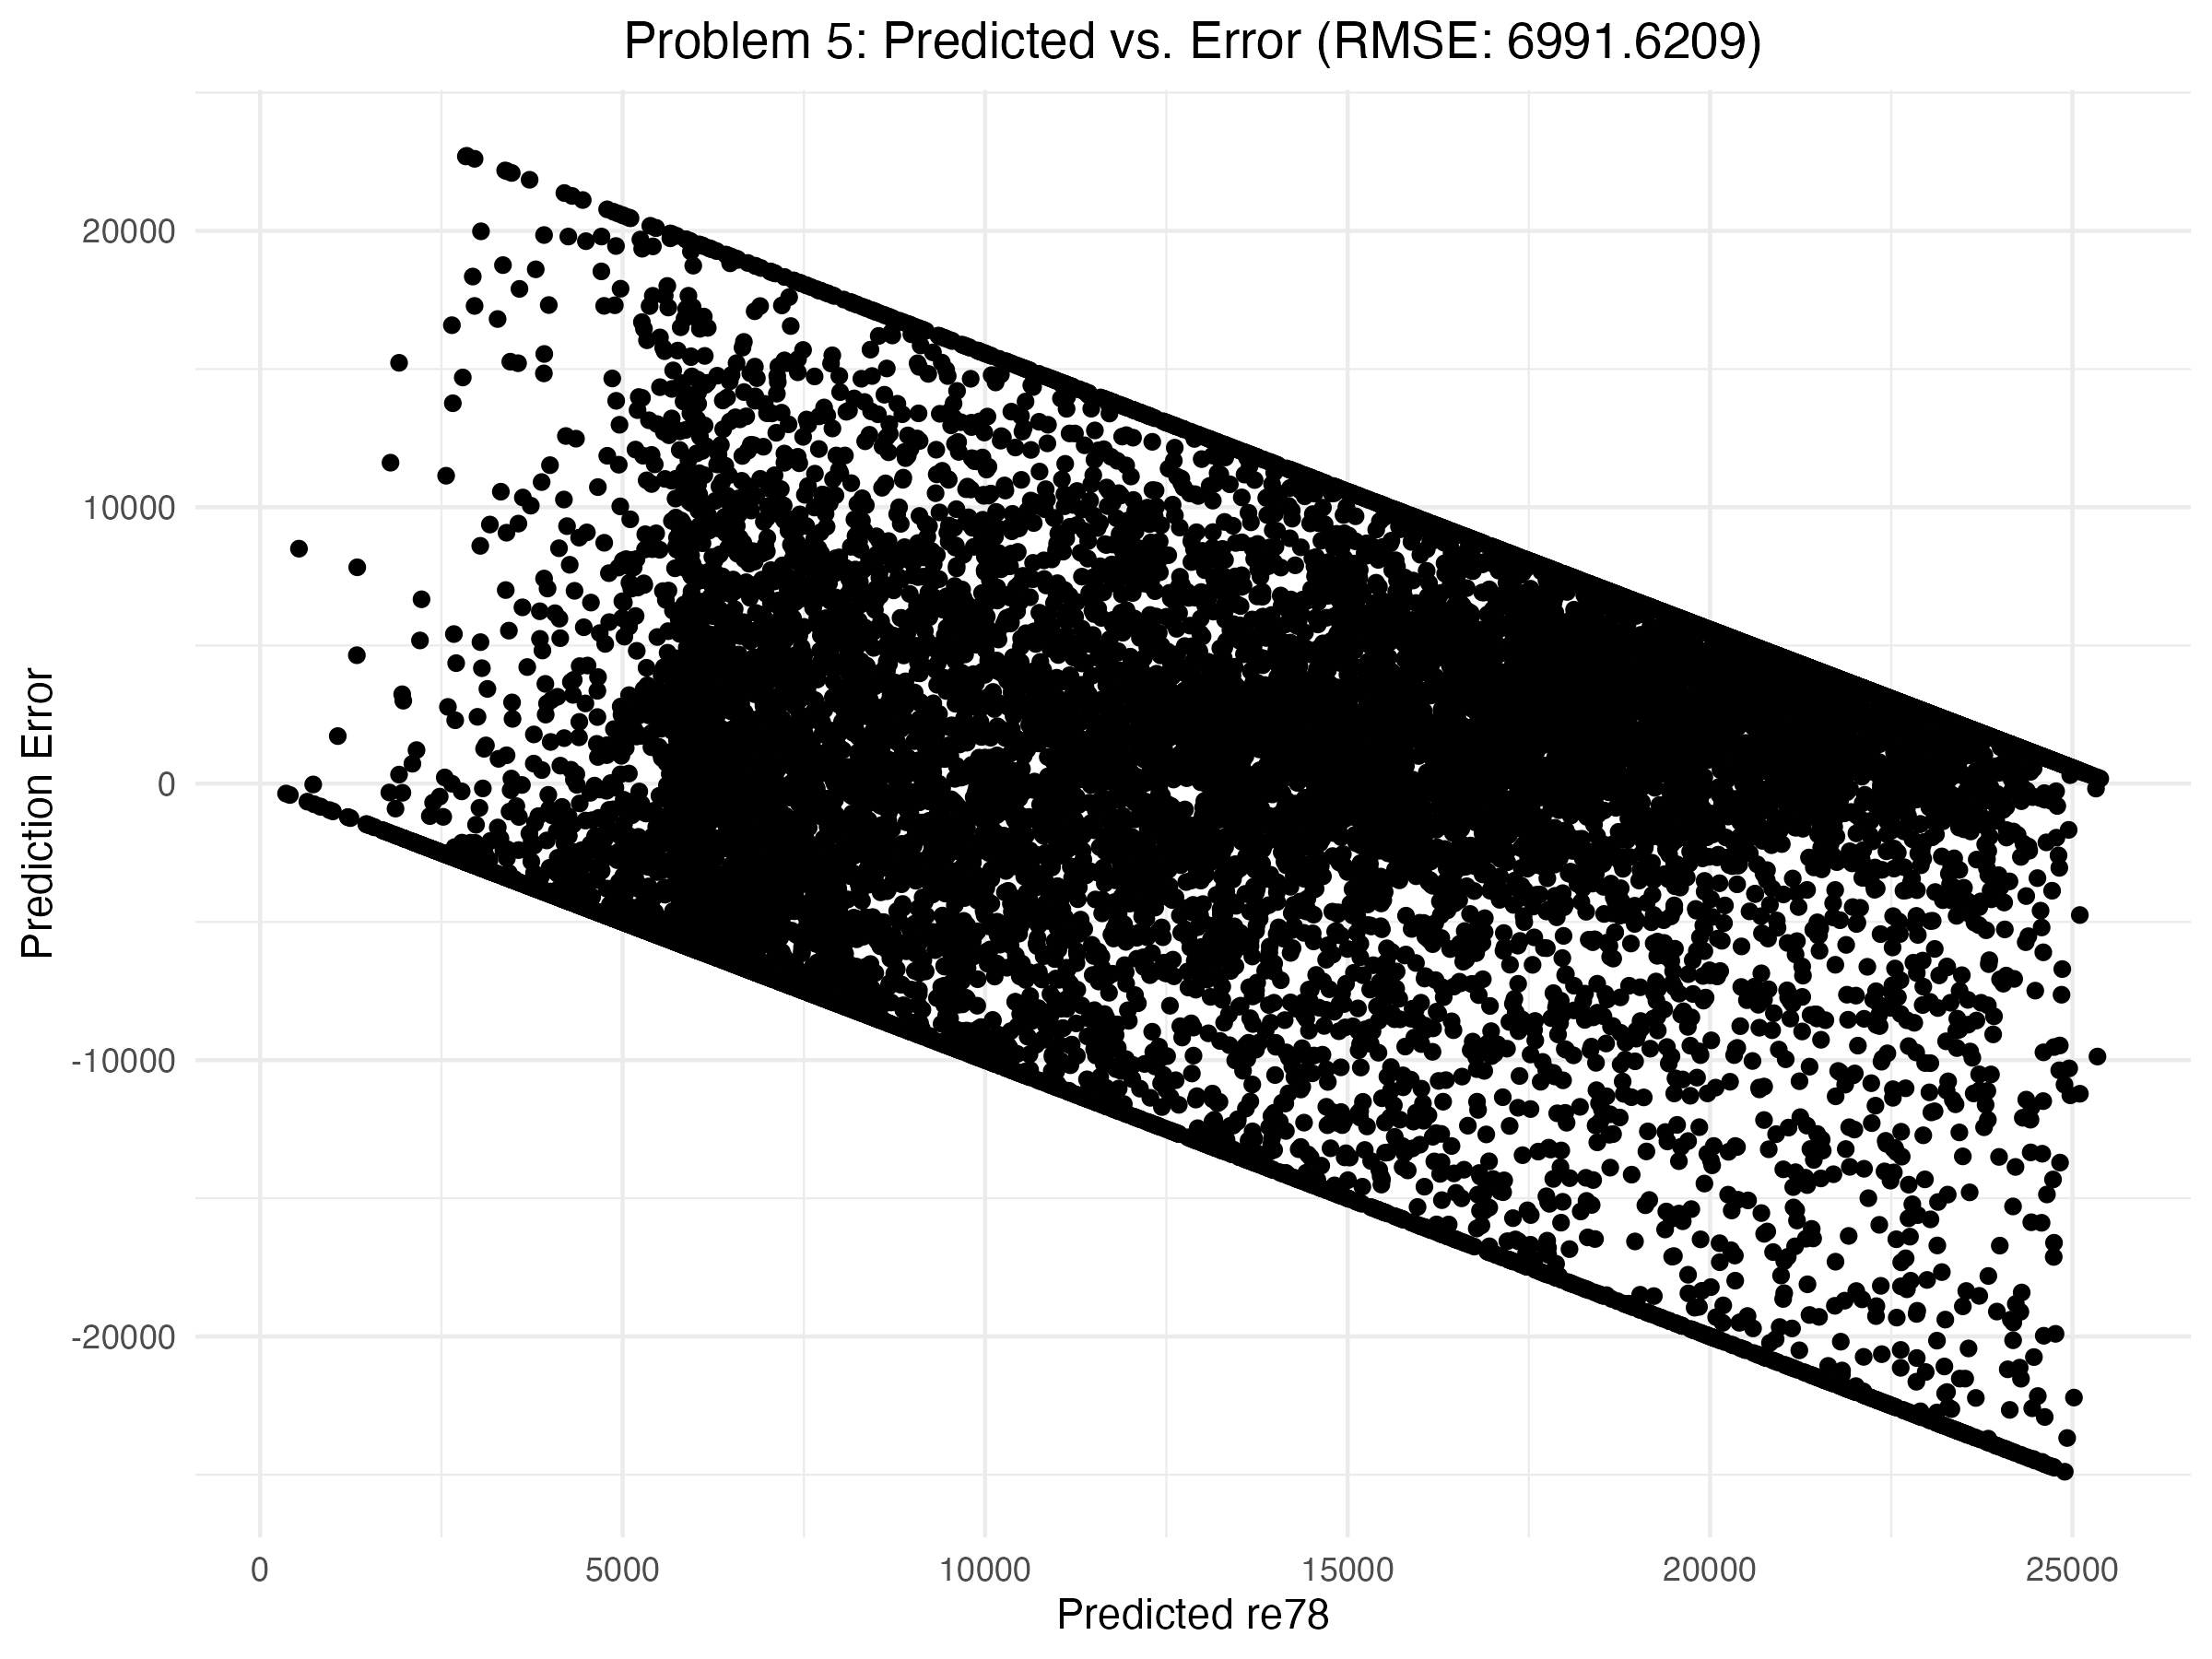
\includegraphics[width=0.8\textwidth]{output/scatterplot_predicted_re78_error_p5_cv.png}
    \caption{\label{fig:scatterplot_predicted_re78_error_p5_cv}Scatterplot of predicted re78 and error}
\end{figure}



\appendix
\setcounter{figure}{0}                      
\setcounter{table}{0}                      
\renewcommand\thefigure{A.\arabic{figure}} 
\renewcommand\thetable{A.\arabic{table}} 


\newpage

\section{Summary Statistics}
\begin{sidewaystable}[h]
    \centering
    \tiny
    
\begin{tabular}{lrrrrrrrrrrrrrrrr}
\toprule
variable & numNA & numZeros & fracZeros & mean & sd & min & max & 10\% & 20\% & 30\% & 40\% & 50\% & 90\% & 95\% & 99\% & 99.9\%\\
\midrule
treat & 0 & 15,992 & 1.0000 & 0.0000 & 0.0000 & 0 & 0.00 & 0.0 & 0.000 & 0.000 & 0.00 & 0.00 & 0.00 & 0.00 & 0.00 & 0.00\\
age & 0 & 0 & 0.0000 & 33.2252 & 11.0452 & 16 & 55.00 & 19.0 & 23.000 & 26.000 & 28.00 & 31.00 & 50.00 & 53.00 & 55.00 & 55.00\\
education & 0 & 36 & 0.0023 & 12.0275 & 2.8708 & 0 & 18.00 & 8.0 & 10.000 & 12.000 & 12.00 & 12.00 & 16.00 & 17.00 & 18.00 & 18.00\\
black & 0 & 14,816 & 0.9265 & 0.0735 & 0.2610 & 0 & 1.00 & 0.0 & 0.000 & 0.000 & 0.00 & 0.00 & 0.00 & 1.00 & 1.00 & 1.00\\
hispanic & 0 & 14,840 & 0.9280 & 0.0720 & 0.2586 & 0 & 1.00 & 0.0 & 0.000 & 0.000 & 0.00 & 0.00 & 0.00 & 1.00 & 1.00 & 1.00\\
\addlinespace
married & 0 & 4,610 & 0.2883 & 0.7117 & 0.4530 & 0 & 1.00 & 0.0 & 0.000 & 1.000 & 1.00 & 1.00 & 1.00 & 1.00 & 1.00 & 1.00\\
nodegree & 0 & 11,261 & 0.7042 & 0.2958 & 0.4564 & 0 & 1.00 & 0.0 & 0.000 & 0.000 & 0.00 & 0.00 & 1.00 & 1.00 & 1.00 & 1.00\\
re74 & 0 & 1,913 & 0.1196 & 14,016.8003 & 9,569.7959 & 0 & 25,862.32 & 0.0 & 2,411.857 & 6,716.955 & 11,207.01 & 15,123.58 & 25,862.32 & 25,862.32 & 25,862.32 & 25,862.32\\
re75 & 0 & 1,748 & 0.1093 & 13,650.8034 & 9,270.4032 & 0 & 25,243.55 & 0.0 & 2,544.406 & 6,565.650 & 10,994.37 & 14,557.11 & 25,243.55 & 25,243.55 & 25,243.55 & 25,243.55\\
re78 & 0 & 2,172 & 0.1358 & 14,846.6597 & 9,647.3915 & 0 & 25,564.67 & 0.0 & 2,915.850 & 8,198.427 & 12,814.25 & 16,421.97 & 25,564.67 & 25,564.67 & 25,564.67 & 25,564.67\\
\addlinespace
id & 0 & 0 & 0.0000 & 7,996.5000 & 4,616.6371 & 1 & 15,992.00 & 1,600.1 & 3,199.200 & 4,798.300 & 6,397.40 & 7,996.50 & 14,392.90 & 15,192.45 & 15,832.09 & 15,976.01\\
\bottomrule
\end{tabular}

    \caption{\label{tab:summary_stats}Summary Statistics}
\end{sidewaystable}


\begin{figure}[h]
    \centering
    
\includegraphics[width=\textwidth]{output/scatterplot_matrix.png}
    \caption{\label{fig:scatterplot_matrix}Scatterplot Matrix}
\end{figure}

\begin{figure}[h]
    \centering
    
\includegraphics[width=\textwidth]{output/correlation_matrix_plot.png}
    \caption{\label{fig:correlation_matrix_plot}Correlation Matrix Plot}
\end{figure}



\end{document}